\documentclass[border=10pt]{standalone}
\usepackage{tikz}
\usetikzlibrary{matrix}

\begin{document}
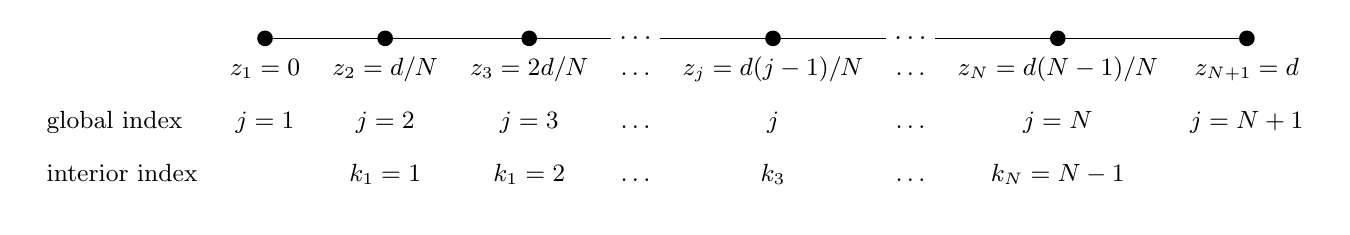
\begin{tikzpicture}
\matrix[
    matrix of math nodes, 
    nodes={text depth=.25em, text height=1em}, 
    font=\small, 
    column 1/.style={anchor=base west}, 
    column sep=5pt
] (m) {
%
    & z_1 = 0 & z_2 = d/N & z_3 = 2d/N & \ldots 
    &  z_j = d(j - 1)/N & \ldots 
    & z_N = d(N - 1)/N & z_{N + 1} = d \\
%                           
\textrm{global index} 
    & j = 1 & j = 2 & j = 3 & \ldots 
    & j & \ldots 
    & j = N & j = N + 1 \\
%                           
\textrm{interior index} 
    & & k_1 = 1 & k_1 = 2 & \ldots 
    & k_3 & \ldots 
    & k_N = N - 1 & \\
%
};
\draw (m-1-2.north) -- (m-1-5.north west) 
    (m-1-5.north east) -- (m-1-7.north west)
    (m-1-7.north east) -- (m-1-9.north);
\foreach \x in {2,3,4,6,8,9} {
    \node[circle, fill, inner sep=2pt] at (m-1-\x .north) {};
}
    \node at (m-1-5.north) { $\ldots$ };
    \node at (m-1-7.north) { $\ldots$ };
\end{tikzpicture}
\end{document}